\newpage
\section{Theoretical Analysis}
\label{sec:analysis}

In this section we will discuss the theoretical analysis of our circuit. For this purpose, we will first explain seperately the envelope detector and the voltage regulator circuits on the AC/DC converter. The values used throughout this analysis are shown below. $V_ON$ is achieved by using the Ngspice value for $V_out$. Theoretically, $V_ON$ is given by equation~\ref{eq:eqvon}.

\begin{equation}
  V_{ON} = \frac{V_{out}}{N_{diodes}},
  \label{eq:eqvon}
\end{equation}

$V_{ON}$ value is computed using \textit{Ngspice} results for $V_{out}$. By definition, $V_{ON}=\frac{V_{out}}{N_{diodes}}$
\begin{table}[h]
    \centering
    \begin{tabular}{|l|c|}
    \hline
    {\bf Symbol} & {\bf Value} \\ \hline
    $V_{ON}$ & $988745938$ \\ \hline
    $A_f$ & $14.64891221288435 V$ \\ \hline
    $R_{ef}$ & $26 k\Omega$  \\ \hline
    $R_{rf}$ & $10 k\Omega$\\ \hline
    $C$ & $3.3750e-05 F$ \\ \hline
    $n$\footnotemark & $20$  \\ \hline
    $\eta$ & $1$  \\ \hline
    \end{tabular}
    \caption{Values for theoretical analysis}
    \label{tab:values}
\end{table}

\footnotetext{This refers to the n constant in the transformer.}

\subsection{Envelope Detector}
\label{sec:envelope}

\begin{figure}[!ht] \centering
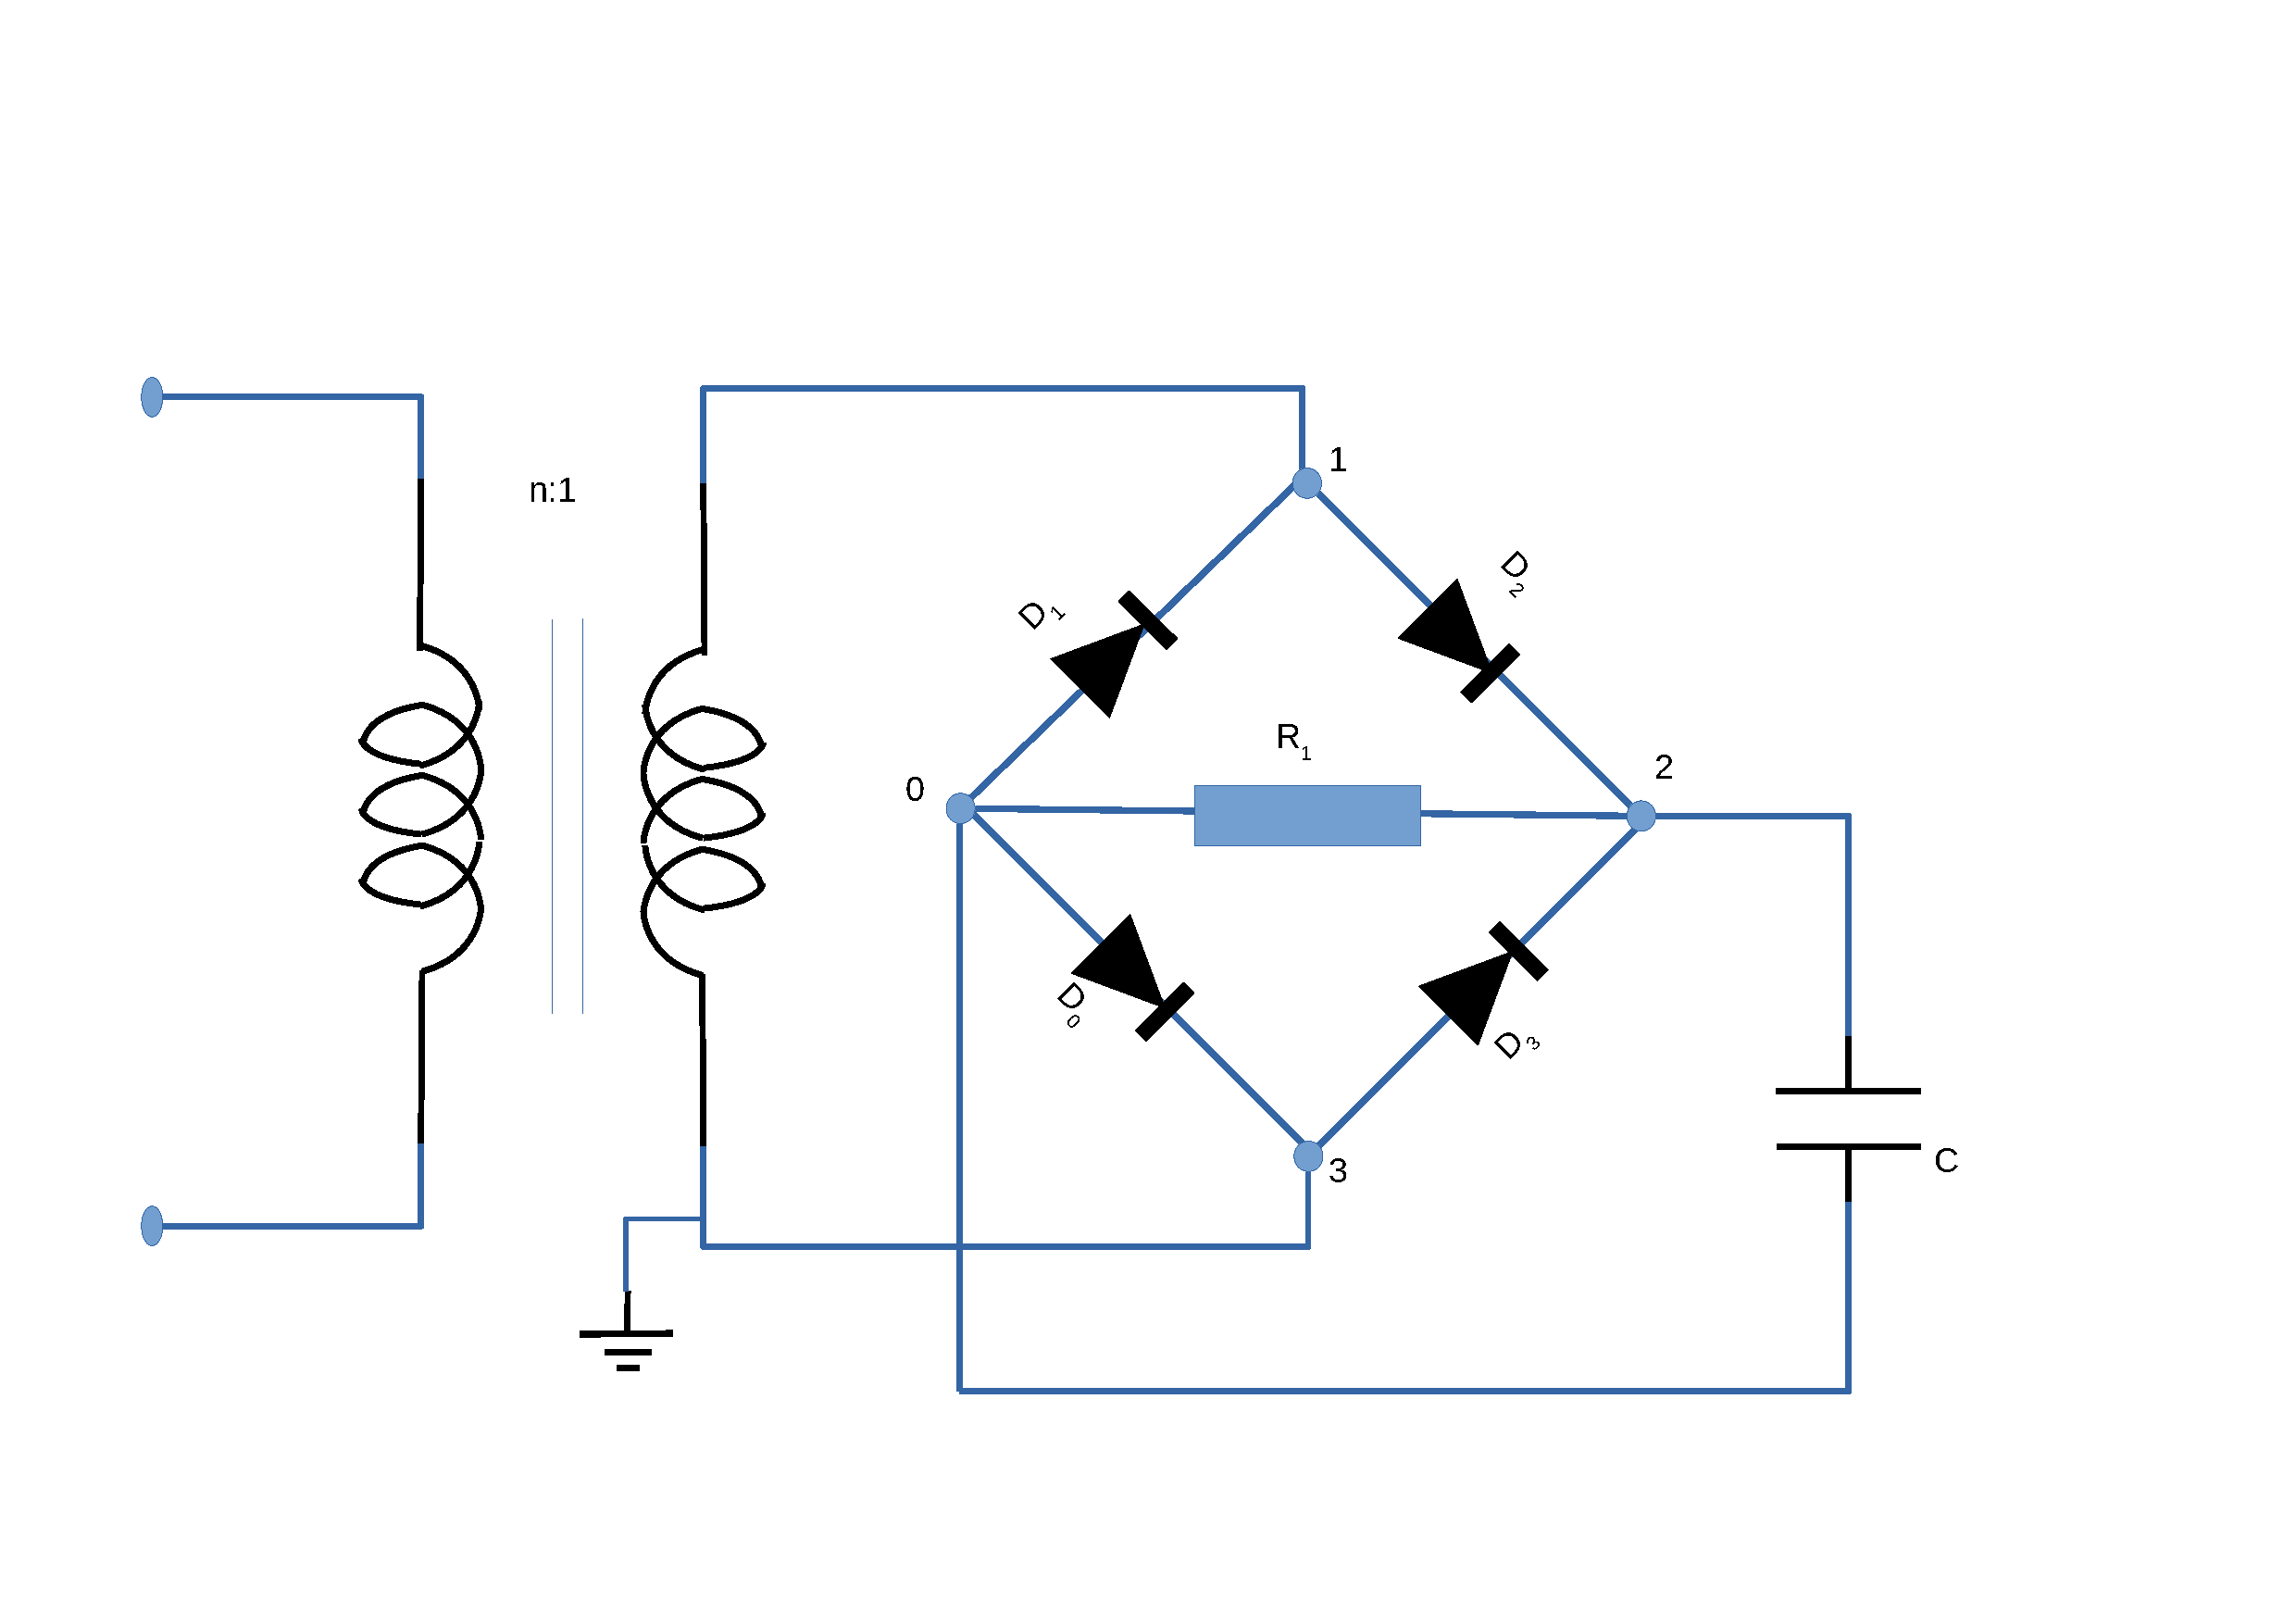
\includegraphics[width=0.8\linewidth]{envelopedetector.pdf} %por aqui figura
\squeezeup 
\caption{Envelope Detector Circuit.}
\label{fig:envelope}
\end{figure}

As seen in figure \ref{fig:envelope}, the envelope detector part of the circuit consists on a full wave bridge rectifier, a resistor ($R_ef$) and a capacitator ($C$), the last two in paralell. To reach the mininum ripple possible, we can increase the resistor impedance and the capacitor capacity, so that the time constant $\tau$ of the capacitor discharge is high enough ($\tau=RC$). Another method was to use a full wave rectifier, as said above, since the time of discharge of $C$ is half of what it would be using a half wave rectifier. This part of the circuit was used to envelope the $V_{in}$ sinusoidal wave, being $V_{in}$ achieved from the following equation.

The envelope detector can be on a positive cycle where $D_0$ and $D_2$ let current pass or a negative cycle that corresponds to $D_1$ and $D_3$ letting the current pass.
\begin{equation}
  V_{in} = \frac{230V}{n},
  \label{eq:vin}
\end{equation}
 
Regardless of the cicle the envelope detector is on, using KVL we achieve the following equation.

\begin{equation}
    V_o + 2V_{ON} - V_{in} = 0,
 \label{eq:envelope2}  
\end{equation}

When the current on the resistor is equal to the current on the capacitor, the diodes shut off, leading to the following equation.

%EQUACAO COPIADA NAO SEI SE ESTA CERTA

\begin{equation}
    \frac{Acos(\omega t|_{OFF})-2V_{ON}}{R_{eq}}=A\omega sin(\omega t|_{OFF})
\end{equation}
where $R_{eq}=R_{env}||R_{vreg}$

\begin{equation}
    V_o=V_o|_{t_{OFF}}e^{-\frac{t-t_{OFF}}{R_{eq}C}}
\end{equation}


\subsection{Voltage Regulator}
\label{sec:regulator}

\begin{figure}[h]
    \centering
    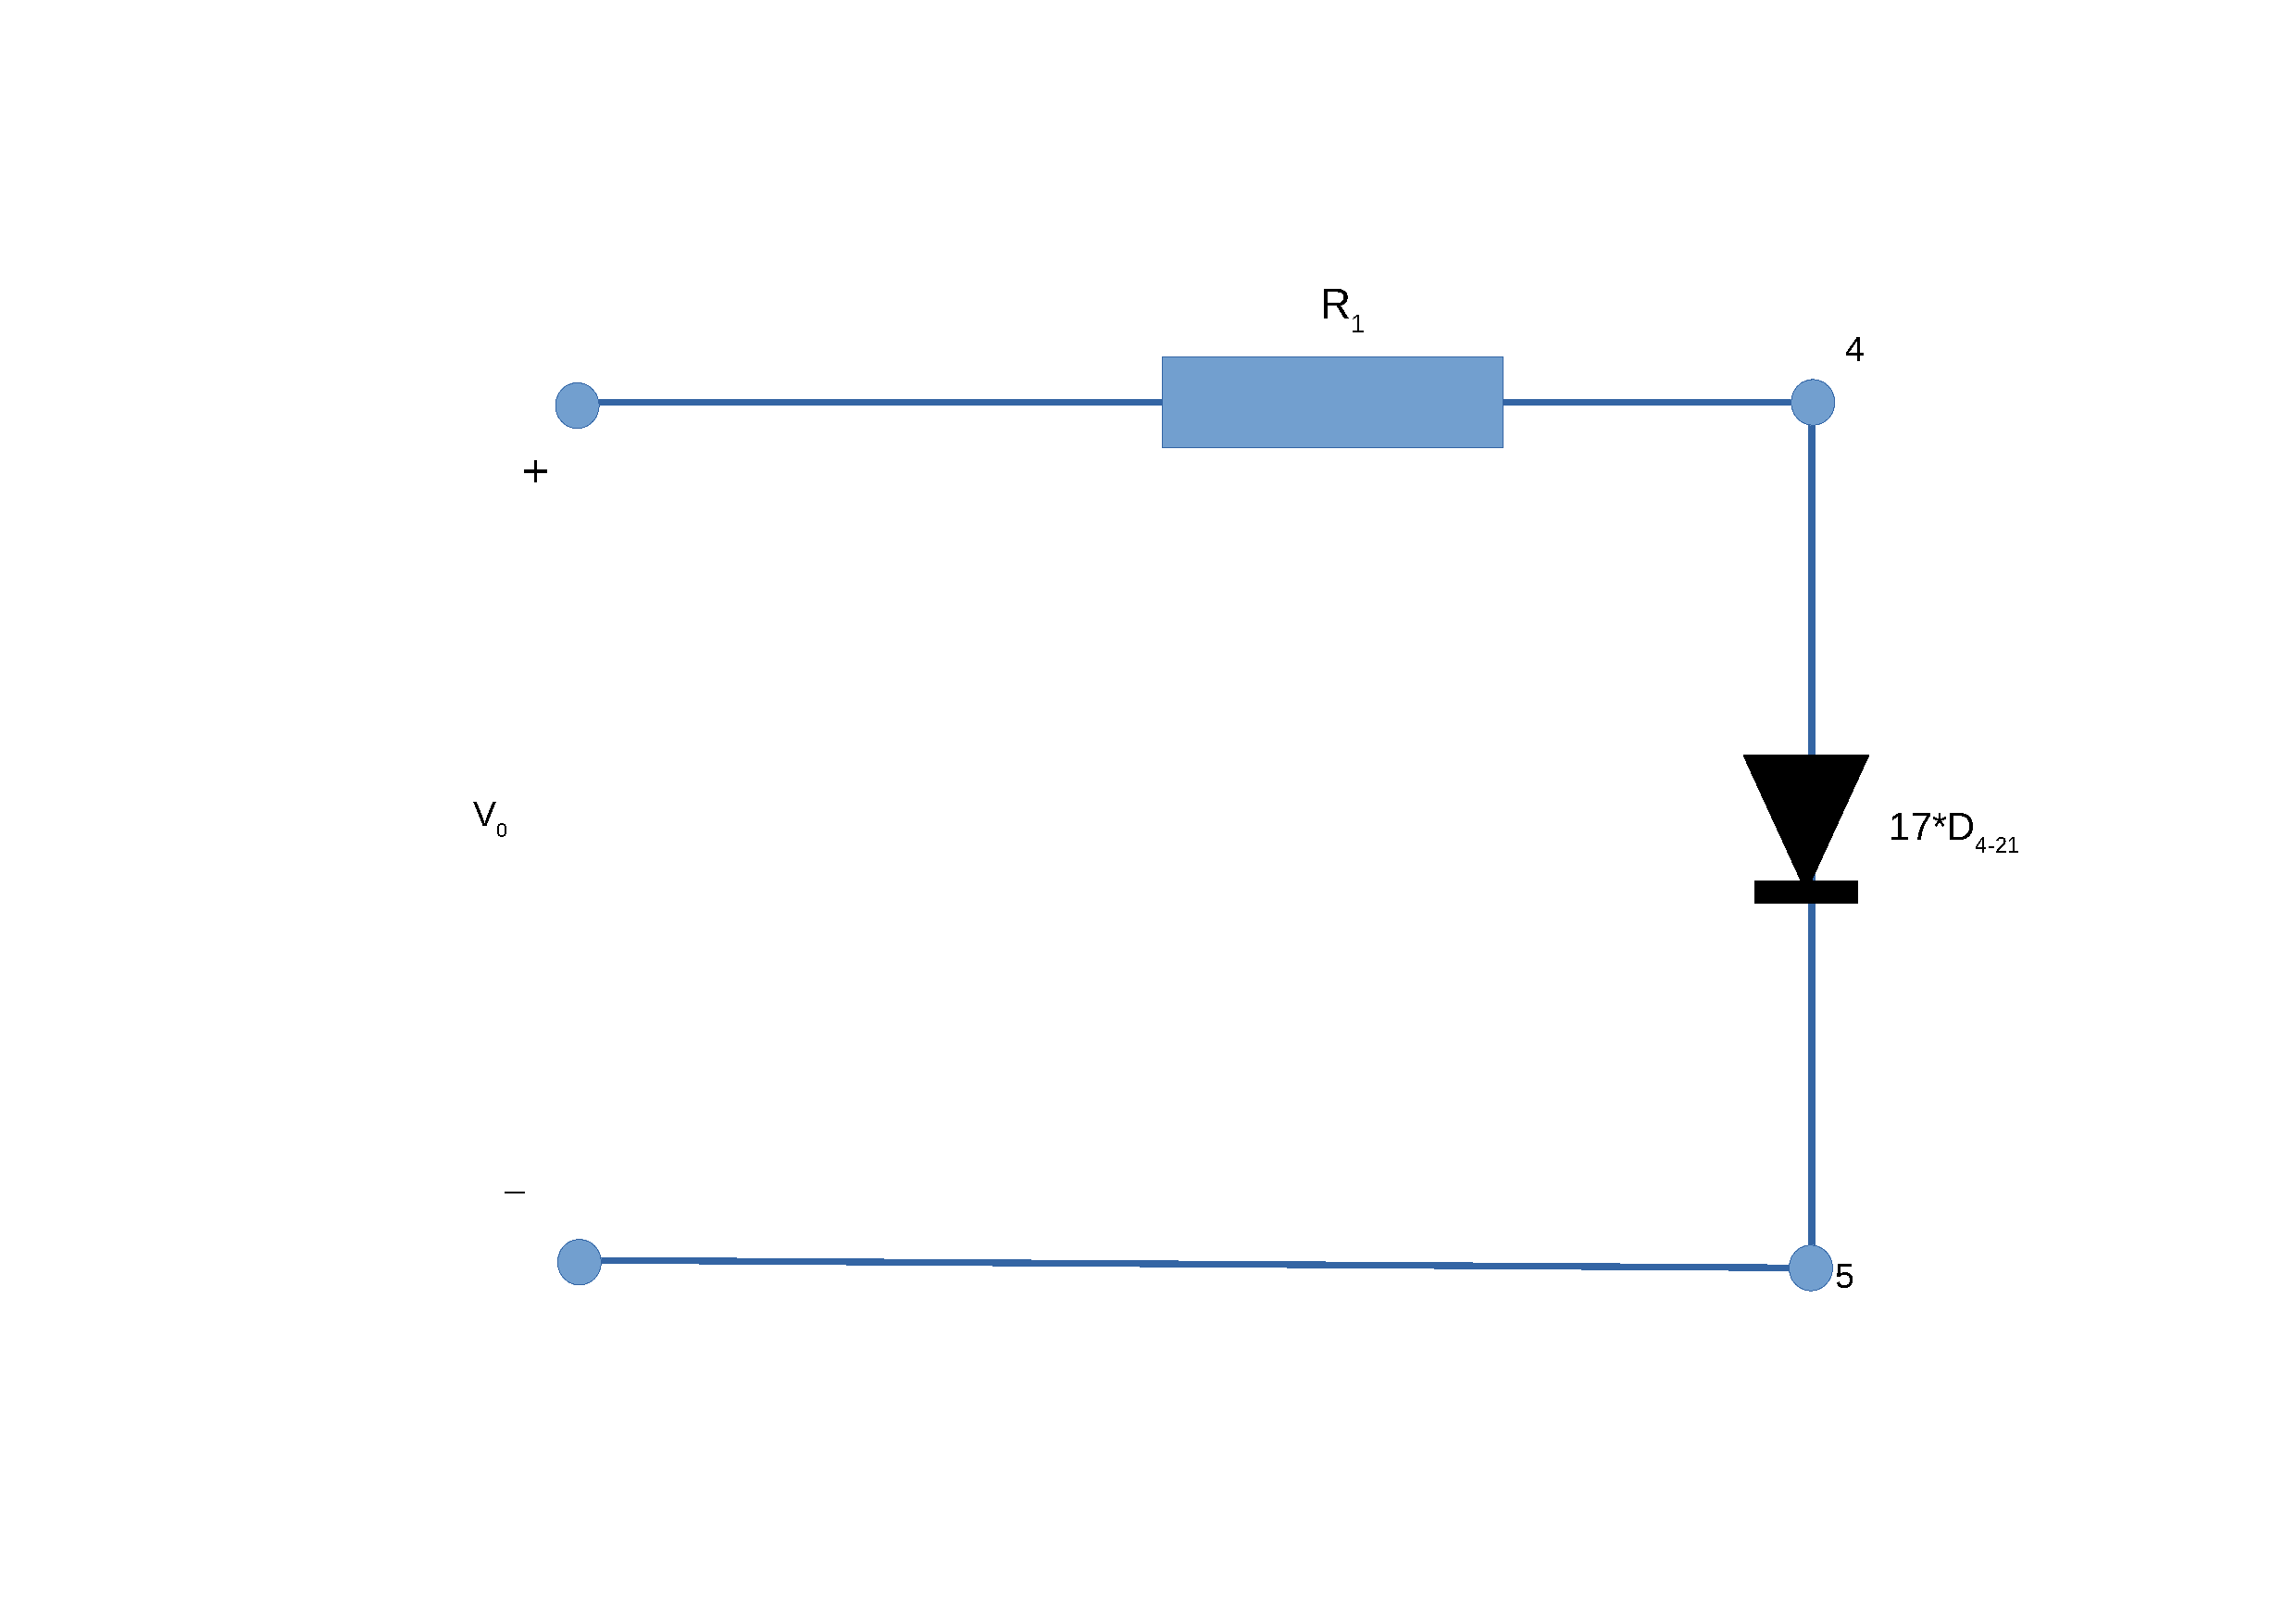
\includegraphics[scale=0.5]{voltageregulator.pdf}
    \caption{Voltage Regulator Circuit.}
    \label{fig:Regulator}
\end{figure}

This part of this circuit was implemented so as to limit the voltage value and to soften the riple of the voltage that came from the previous part of the circuit (\ref{sec:envelope}). It involves a resistor and seventeen diodes in series.

%COPIADO NAO SEI REESCREVER ISTO, NAO PERCEBO NADA DESCULPEM  (parte em baixo)

The analysis has to be made by seperating the DC and AC components. The DC simulation uses the condition $V_o=N * V_{ON}$, so that we can replace each diode with $V_{ON}$. 

In this section, the theoretical analysis requires we think about the DC and AC components separately ($V_o=V_O+v_o$). 

The DC analysis is fairly simple since if $V_O>17*V_{ON}$, $V_O$ is equal to $17*V_{ON}$. The number 17 can be replaced by any number of diodes chosen. 

As for AC, we achieve equation \ref{eq:Ac1} by using equations \ref{eq:Ac2} and \ref{eq:Ac3}. The variable $k$ is the Boltzmann constant, $T$ is the temperature in Kelvin and $q$ is electron charge. To lower the $v_{out}$ ripple, the value for $r_d$ should also be low (see equation \ref{eq:Ac2}).

\begin{equation}
    v_{out}=\frac{n r_{d}}{n r_{d} + R_{vreg}}v_o,
    \label{eq:Ac1}
\end{equation}

\begin{equation}
    r_{d}=\frac{\eta V_T}{I_s e^{\frac{V_D}{\eta V_T}}},
    \label{eq:Ac2}
\end{equation}

\begin{equation}
    V_{T} = \frac{kT}{q},
    \label{eq:Ac3}
\end{equation}

\newpage 

\newpage 




